\UseRawInputEncoding
%% ReflectiveTun — Automation in Construction (cas-dc double-column template)

\documentclass[a4paper,fleqn]{cas-dc}

\usepackage[numbers]{natbib}
\usepackage{booktabs}
\usepackage{multirow}
\usepackage{amsmath}
\usepackage{amssymb} % for \checkmark, \circlearrowright
\usepackage{algorithm}
\usepackage{algpseudocode}
\usepackage{graphicx}
\usepackage[dvipsnames]{xcolor}
\usepackage{hyperref}
\usepackage{placeins}
\usepackage{flafter} % prevent floats from appearing before their definition
\usepackage{float} % provides [H] to force a float to appear exactly here
\usepackage{caption}
\usepackage{subcaption} % provides subfigure environment
\usepackage{balance}
\usepackage{tikz}
\usetikzlibrary{arrows.meta,positioning,calc,fit}

% ─── Shared TikZ styles (reused across figures) ────────────────────────────
\tikzset{%
  box/.style={draw,rounded corners,align=center,minimum height=8mm,inner sep=4pt},
  gate/.style={draw,rounded corners,align=center,minimum height=10mm,inner sep=5pt},
  arrow/.style={-{Latex[length=2mm]}, thick}%
}

\usepackage{soul} % for \\hl
% Allow soul highlighting to contain common cross-reference commands
\soulregister\ref7
\soulregister\pageref7
\soulregister\eqref7
% Highlight helper that also works in math mode (e.g., $+36\%$)
\newcommand{\hlpct}[1]{\ifmmode\mbox{\hl{#1}}\else\hl{#1}\fi}
\usepackage{tcolorbox} % for section-wide highlighting

\providecommand{\printorcid}{}
\providecommand{\printfacebook}{}
\providecommand{\printtwitter}{}
\providecommand{\printlinkedin}{}
\providecommand{\printgplus}{}
\providecommand{\printinstagram}{}
\providecommand{\printemails}{}
\providecommand{\printurls}{}
\usepackage{lineno}
%\linenumbers % (disabled)

\begin{document}
\let\WriteBookmarks\relax
\def\floatpagepagefraction{1}
\def\textpagefraction{.001}

% ────────────────────────────── Front matter ──────────────────────────────

{\shorttitle{Proxy4Tun: self-refine deployment-label-free tunnel point-cloud segmentation}
\shortauthors{X.\ Tao et~al.}

\title[mode=title]{Proxy4Tun: self-refine framework for deployment-label-free segmental tunnel lining segmentation}

\author[1]{Xinghui Tao}
\credit{Conceptualization, Methodology, Software, Writing -- original draft}

\author[1]{Guangming Wang}
\cormark[1]
\ead{gw462@cam.ac.uk}
\credit{Supervision, Writing -- review \& editing}

\author[1]{Brian Sheil}
\credit{Supervision, Funding acquisition, Project administration}

\cortext[cor1]{Corresponding author}

\affiliation[1]{organization={Construction Engineering, University of Cambridge},
    addressline={Trumpington Street},
    city={Cambridge},
    postcode={CB2 1PZ},
    country={United Kingdom}}

% ─── Abstract ─────────────────────────────────────────────────────────────


\begin{abstract}
Segment-wise inspection of tunnel linings, such as joint gaps, leakage, and deformation, requires accurate segmentation, yet deployment rarely provides ground-truth labels for tuning or quality control. We present \textbf{Proxy4Tun}, a deployment-time, label-free assess-and-refine framework for a projection-based, ring-level pipeline. At design time, Bayesian optimisation (BO) on a small set of Labelled diversity-selected rings selects a bounded set of sensitive parameters and a compact set of intrinsic metrics that correlate with mIoU; these are then used to learn a proxy objective that guides deployment-time self-refinement. We also address a ring-level projection failure mode in which rotational ambiguity produces physically misaligned segmentations. We mitigate this with a gravity-referenced bottom-alignment prior applied before refinement. On 50 evaluation rings from 17 Seg2Tunnel sections, mean IoU increases by 346\% (from 0.109 to 0.412) with bottom alignment and proxy-guided refinement. These results indicate that calibrated intrinsic proxies can support label-free adaptation and quality control at deployment.
\end{abstract}


% ─── Highlights ───────────────────────────────────────────────────────────

\begin{highlights}
\item Label-free point cloud tunnel-lining segmentation at deployment.
\item Ring-level projection-based pipeline employing boundary detection.
\item Design-time BO-calibrated intrinsic proxy serving as an mIoU indicator.
\item Self-refinement increases mean mIoU by 3.46-fold compared with SAM4Tun.
\end{highlights}

% ─── Keywords ─────────────────────────────────────────────────────────────

\begin{keywords}
Tunnel-lining segmentation \sep Point-cloud segmentation \sep Depth-map segmentation \sep Deployment-time self-refinement \sep Intrinsic proxy \sep Bayesian optimisation
\end{keywords}

\maketitle

\smallskip
% ─────────────────────────────────────────────────────────────────────────

% ══════════════════════════════════════════════════════════════════════════
\section{Introduction}\label{sec:intro}
% ══════════════════════════════════════════════════════════════════════════
% ─── Figure (TikZ): Motivation and positioning ────────────────────────────
\begin{figure*}[t]
\centering

% ---------------- Panel (a) ----------------
\begin{subfigure}{0.98\textwidth}
\centering
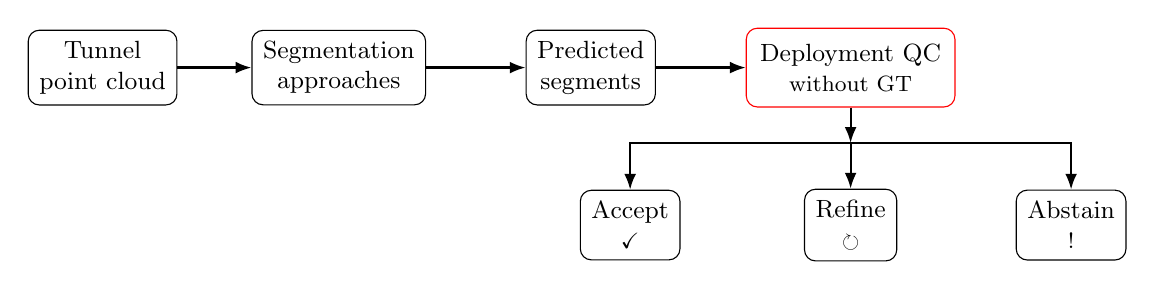
\begin{tikzpicture}[
    font=\small
]

% Main horizontal flow
\node[box] (ring) at (0,0) {Tunnel \\ point cloud};
\node[box] (seg) at (3.0,0) {Segmentation\\approaches};
\node[box] (layout) at (6.2,0) {Predicted\\segments};
\node[gate, draw=red] (qc) at (9.5,0) {Deployment QC \\{\footnotesize without GT}};

\draw[arrow] (ring) -- (seg);
\draw[arrow] (seg) -- (layout);
\draw[arrow] (layout) -- (qc);

% Decision outputs
\coordinate (fork) at ($(qc.south)+(0,-0.45)$);
\draw[arrow] (qc.south) -- (fork);

\node[box] (accept) at (6.7,-2.0) {Accept\\{\footnotesize $\checkmark$}};
\node[box] (refine) at (9.5,-2.0) {Refine\\{\footnotesize $\circlearrowright$}};
\node[box] (abstain) at (12.3,-2.0) {Abstain\\{\footnotesize !}};

\draw[arrow] (fork) -| (accept.north);
\draw[arrow] (fork) -- (refine.north);
\draw[arrow] (fork) -| (abstain.north);

\end{tikzpicture}
\caption{Deployment decision gap.}
\end{subfigure}

\vspace{4mm}

% ---------------- Panel (b) ----------------
\begin{subfigure}{0.98\textwidth}
\centering
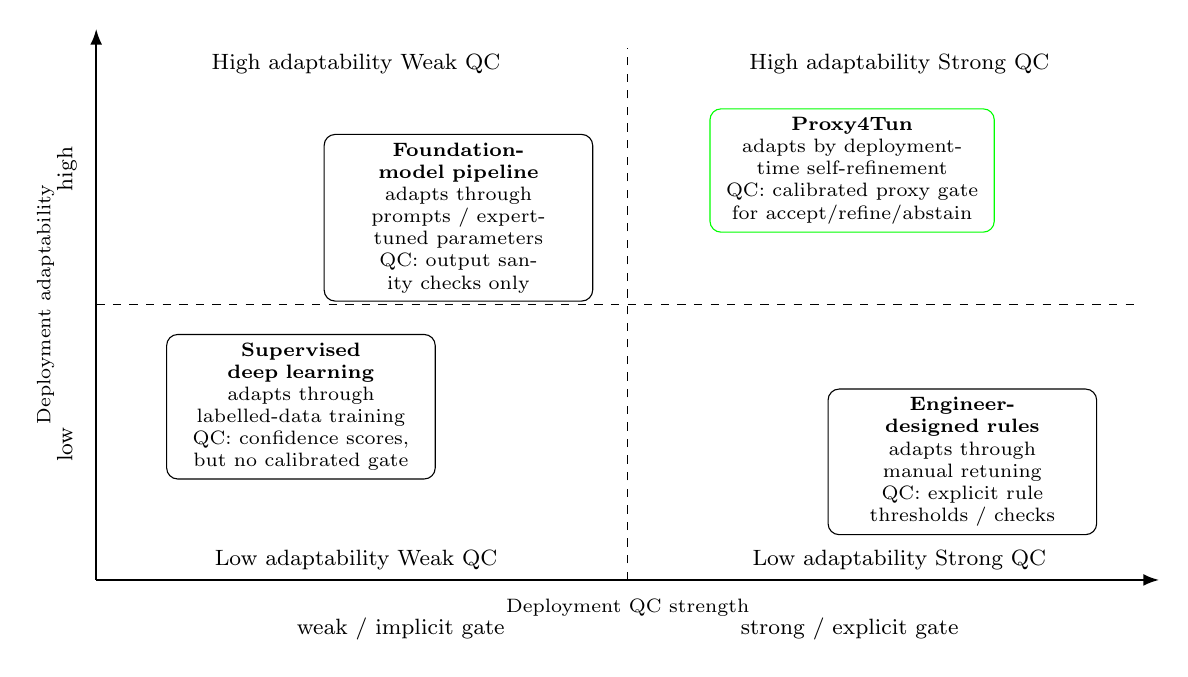
\begin{tikzpicture}[
    font=\scriptsize,
    method/.style={
        draw,
        rounded corners,
        align=center,
        text width=32mm,
        inner sep=3pt
    },
    proxy/.style={
        draw,
        rounded corners,
        align=center,
        text width=34mm,
        inner sep=3pt
    },
    axis/.style={-{Latex[length=2mm]}, thick},
    guide/.style={dashed, thin}
]

% Axes (slightly larger canvas to avoid overlaps)
\draw[axis] (0,0) -- (13.5,0);
\draw[axis] (0,0) -- (0,7.0);

% Middle guide lines
\draw[guide] (6.75,0) -- (6.75,6.75);
\draw[guide] (0,3.5) -- (13.2,3.5);

% Axis labels
\node[align=center] at (6.75,-0.5)
{Deployment QC strength\\
{\footnotesize weak / implicit gate \hspace{28mm} strong / explicit gate}};

\node[rotate=90, align=center] at (-0.5,3.5)
{Deployment adaptability\\
{\footnotesize low \hspace{28mm} high}};

% Quadrant labels (pushed outward so they don't collide with boxes)
\node[align=center, font=\footnotesize] at (3.3,6.55) {High adaptability Weak QC};
\node[align=center, font=\footnotesize] at (10.2,6.55) {High adaptability Strong QC};
\node[align=center, font=\footnotesize] at (3.3,0.25) {Low adaptability Weak QC};
\node[align=center, font=\footnotesize] at (10.2,0.25) {Low adaptability Strong QC};

% Method boxes (spread out a bit)
\node[proxy, draw=green] (proxy4tun) at (9.6,5.2)
{\textbf{Proxy4Tun}\\
adapts by deployment-time self-refinement\\
QC: calibrated proxy gate for accept/refine/abstain\\
};

\node[method] (fm) at (4.6,4.6)
{\textbf{Foundation-model pipeline}\\
adapts through prompts / expert-tuned parameters\\
QC: output sanity checks only};

\node[method] (dl) at (2.6,2.2)
{\textbf{Supervised}\\
\textbf{deep learning}\\
adapts through labelled-data training\\
QC: confidence scores, but no calibrated gate};

\node[method] (rules) at (11.0,1.5)
{\textbf{Engineer-designed rules}\\
adapts through manual retuning\\
QC: explicit rule thresholds / checks\\
};

\end{tikzpicture}
\caption{Conceptual approach positioning under deployment constraints.}
\end{subfigure}

\caption{
Motivation and positioning of Proxy4Tun.
(a) At deployment, tunnel-ring segmentation outputs require accept, refine, or abstain decisions without ground truth (GT).
(b) Existing segmentation approaches differ in deployment adaptability and deployment quality-control (QC) strength. Proxy4Tun targets the high-adaptability and strong-QC region by using an intrinsic proxy learnt at design time on a small set of labelled diversity-selected rings, then used for deployment-time scoring and refinement without GT.
}
\label{fig:proxy4tun_motivation_positioning}
\end{figure*}




% ══════════════════════════════════════════════════════════════════════════
\FloatBarrier % keep Fig.~1 with the Introduction (avoid large blank space)
\section{Related work}\label{sec:related}
% ══════════════════════════════════════════════════════════════════════════




% ══════════════════════════════════════════════════════════════════════════
\section{Methodology}\label{sec:methods}
% ══════════════════════════════════════════════════════════════════════════

% ─── Figure (TikZ): Overall Proxy4Tun framework ───────────────────────────
\begin{figure*}[t]
\centering

% ===================== Panel (a): Design time =====================
\begin{subfigure}{0.98\textwidth}
\raggedright

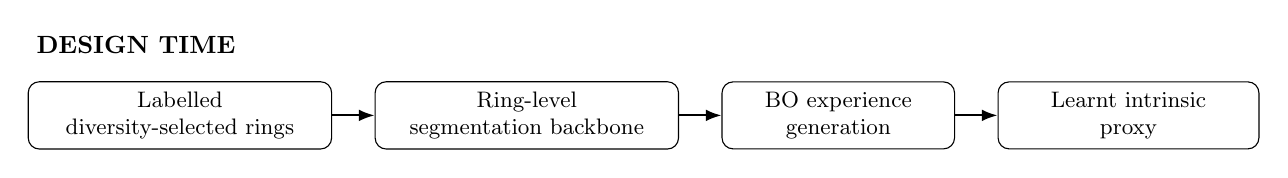
\begin{tikzpicture}[
    font=\small,
    scale=0.9,
    transform shape,
    box/.style={
        draw,
        rounded corners,
        align=center,
        minimum height=8mm,
        text width=30mm,
        inner sep=4pt
    },
    keybox/.style={
        draw,
        rounded corners,
        align=center,
        minimum height=8mm,
        text width=34mm,
        inner sep=4pt
    },
    arrow/.style={-{Latex[length=2mm]}, thick}
]

% Nodes
\node[box, text width=40mm] (panel) at (0,0) {Labelled\\diversity-selected rings};

% Title label (left-aligned to the left edge of the first box)
\node[anchor=west, font=\bfseries] at ([yshift=10mm]panel.west) {DESIGN TIME};
\node[box, text width=40mm, right=6mm of panel] (backbone) {Ring-level \\ segmentation backbone};
\node[box, right=6mm of backbone] (bo) {BO experience\\generation};
\node[keybox, right=6mm of bo] (proxy) {Learnt intrinsic\\proxy};

% Arrows
\draw[arrow] (panel) -- (backbone);
\draw[arrow] (backbone) -- (bo);
\draw[arrow] (bo) -- (proxy);
% (Deployment box removed)


\end{tikzpicture}%

\caption{Design-time calibration of the intrinsic proxy.}
\end{subfigure}

\vspace{5mm}

% ===================== Panel (b): Deployment time =====================
\begin{subfigure}{0.98\textwidth}
\raggedright

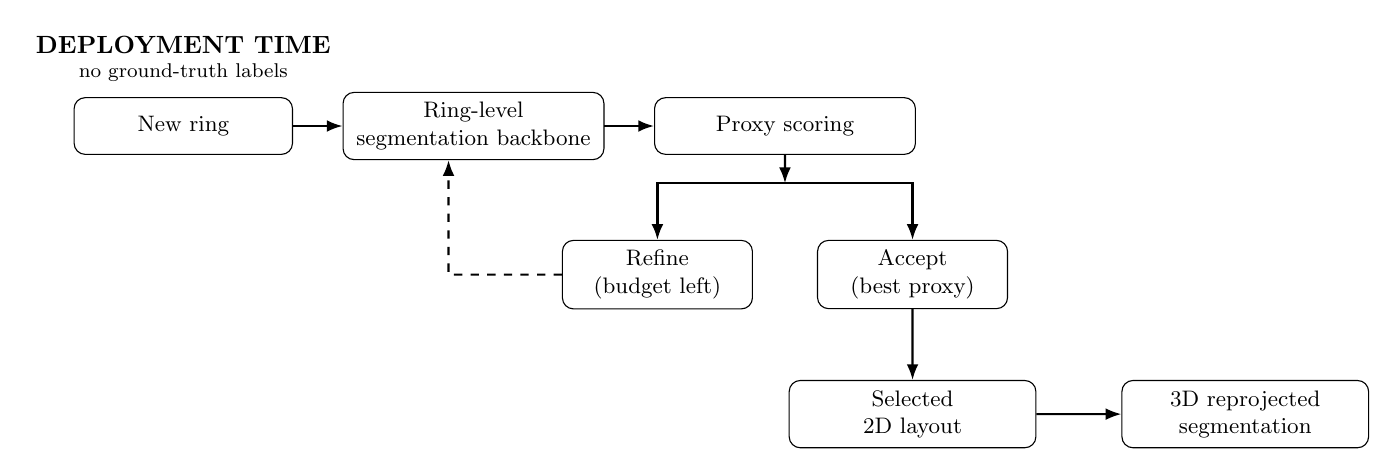
\begin{tikzpicture}[
    font=\small,
    scale=0.9,
    transform shape,
    box/.style={
        draw,
        rounded corners,
        align=center,
        minimum height=8mm,
        text width=28mm,
        inner sep=4pt
    },
    process/.style={
        draw,
        rounded corners,
        align=center,
        minimum height=8mm,
        text width=34mm,
        inner sep=4pt
    },
    decision/.style={
        draw,
        rounded corners,
        align=center,
        minimum height=8mm,
        text width=24mm,
        inner sep=4pt
    },
    finalbox/.style={
        draw,
        rounded corners,
        align=center,
        minimum height=8mm,
        text width=32mm,
        inner sep=4pt
    },
    arrow/.style={-{Latex[length=2mm]}, thick},
    looparrow/.style={-{Latex[length=2mm]}, thick, dashed}
]


% Title label
\node[align=left, font=\bfseries] at (0,1.15) {DEPLOYMENT TIME};
\node[align=left, font=\footnotesize] at (0,0.75) {no ground-truth labels};

% Main runtime pipeline
\node[box] (ring) at (0,0) {New ring};
\node[process, right=7mm of ring] (backbone) {Ring-level\\segmentation backbone};
\node[process, right=7mm of backbone] (score) {Proxy scoring};

\draw[arrow] (ring) -- (backbone);
\draw[arrow] (backbone) -- (score);

% Decision branches (no abstain: accept best when budget ends / improvement plateaus)
% Place decisions centered under the scoring step (Refine left, Accept right).
\node[decision, below=12mm of score, xshift=-18mm] (refine) {Refine\\(budget left)};
\node[decision, below=12mm of score, xshift=18mm] (accept) {Accept\\(best proxy)};

\coordinate (fork) at ($(score.south)+(0,-4mm)$);
\draw[arrow] (score.south) -- (fork);
\draw[arrow] (fork) -| (refine.north);
\draw[arrow] (fork) -| (accept.north);

% Refine loops back towards the ring-level segmentation backbone
% (left, then up; no final rightward segment)
\coordinate (refloopx) at ($(refine.west)+(-16mm,0)$);
\draw[looparrow] (refine.west) -- (refloopx) -- (refloopx |- backbone.south);

% Final output
\node[finalbox, below=10mm of accept] (layout) {Selected\\2D layout};
\node[finalbox, right=12mm of layout] (out3d) {3D reprojected\\segmentation};

\draw[arrow] (accept.south) -- (layout.north);
\draw[arrow] (layout) -- (out3d);

\end{tikzpicture}%

\caption{Deployment-time proxy-guided refinement and selection.}
\end{subfigure}

\caption{
Overall Proxy4Tun framework built around a shared ring-level segmentation backbone used at both design time and deployment.
(a) At design time, six labelled diversity-selected rings are processed by the backbone to generate BO experience and relate intrinsic quality metrics to mIoU, learning an intrinsic proxy.
(b) At deployment, each new ring is stabilised, segmented by the same backbone, and refined through learnt proxy scoring. Refinement continues while budget remains and proxy improvements persist; when the budget is exhausted or improvements plateau, the best proxy-scoring output is accepted (no deployment ground-truth labels).
}
\label{fig:overall_proxy4tun_framework}
\end{figure*}

% ─── Figure (TikZ): Ring-level segmentation backbone ──────────────────────
\begin{figure*}[t]
\centering

% ===================== Panel (a): Ring-level backbone =====================
\begin{subfigure}{0.98\textwidth}
\centering
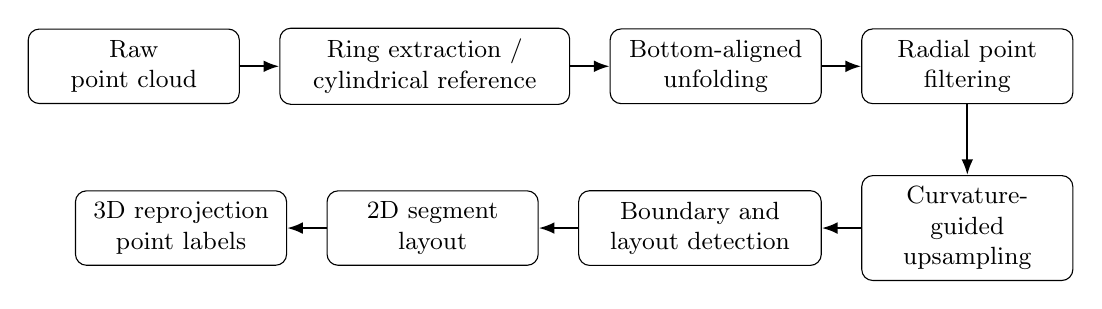
\begin{tikzpicture}[
    font=\small,
    box/.style={
        draw,
        rounded corners,
        align=center,
        minimum height=8mm,
        text width=24mm,
        inner sep=4pt
    },
    keybox/.style={
        draw,
        rounded corners,
        align=center,
        minimum height=8mm,
        text width=28mm,
        inner sep=4pt
    },
    arrow/.style={-{Latex[length=2mm]}, thick}
]

% Nodes (wrapped into two rows to fit page width)
\node[box] (raw) at (0,0) {Raw \\point cloud};
\node[box, text width=34mm, right=5mm of raw] (extract) {Ring extraction /\\cylindrical reference};
\node[box, right=5mm of extract] (unfold) {Bottom-aligned\\unfolding};
\node[box, right=5mm of unfold] (denoise) {Radial point\\filtering};

% Second row flows right-to-left to shorten the denoise→enhance connection
\node[box, below=9mm of denoise] (enhance) {Curvature-guided\\upsampling};
\node[keybox, left=5mm of enhance] (boundary) {Boundary and\\layout detection};
\node[box, left=5mm of boundary] (layout) {2D segment\\layout};
\node[box, left=5mm of layout] (reproj) {3D reprojection\\point labels};

% Arrows
\draw[arrow] (raw) -- (extract);
\draw[arrow] (extract) -- (unfold);
\draw[arrow] (unfold) -- (denoise);
\draw[arrow] (denoise.south) -- (enhance.north);
\draw[arrow] (enhance) -- (boundary);
\draw[arrow] (boundary) -- (layout);
\draw[arrow] (layout) -- (reproj);


\end{tikzpicture}
\caption{Ring-level segmentation backbone.}
\end{subfigure}

\vspace{5mm}

% ===================== Panel (b): Why ring-level =====================
\begin{subfigure}{0.98\textwidth}
\centering
\resizebox{\linewidth}{!}{%
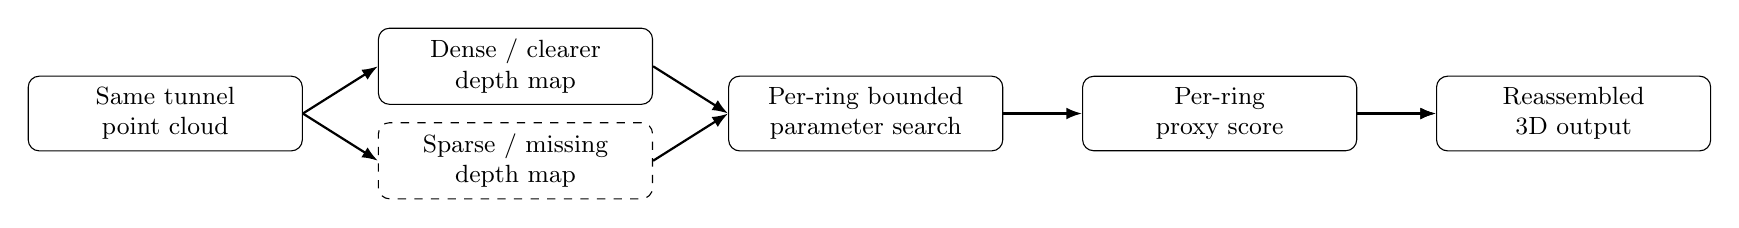
\begin{tikzpicture}[
    font=\small,
    box/.style={
        draw,
        rounded corners,
        align=center,
        minimum height=8mm,
        text width=32mm,
        inner sep=4pt
    },
    good/.style={box},
    bad/.style={box, dashed},
    note/.style={
        draw,
        rounded corners,
        align=left,
        inner sep=5pt,
        text width=150mm,
        font=\footnotesize
    },
    arrow/.style={-{Latex[length=2mm]}, thick}
]

% Input
\node[box] (pc) at (0,0) {Same tunnel\\point cloud};

% Per-ring bounded search + proxy
% (keep the rest of the pipeline vertically centered w.r.t. the input box)
\node[good, right=54mm of pc] (search) {Per-ring bounded\\parameter search};
\node[good, right=10mm of search] (proxy) {Per-ring\\proxy score};
\node[good, right=10mm of proxy] (out) {Reassembled\\3D output};

% Depth maps (heterogeneous quality)
% (place them midway between input and search; split above/below the input midline)
\coordinate (middepth) at ($ (pc.east)!0.5!(search.west) $);
\node[good] (dense)  at ($ (middepth) + (0,6mm) $) {Dense / clearer\\depth map};
\node[bad]  (sparse) at ($ (middepth) + (0,-6mm) $) {Sparse / missing\\depth map};

% Connections
\draw[arrow] (pc.east) -- (dense.west);
\draw[arrow] (pc.east) -- (sparse.west);
\draw[arrow] (dense.east) -- (search.west);
\draw[arrow] (sparse.east) -- (search.west);
\draw[arrow] (search) -- (proxy);
\draw[arrow] (proxy) -- (out);
\draw[arrow] (proxy) -- (out);



\end{tikzpicture}%
}
\caption{Why Proxy4Tun operates at ring level rather than tunnel level.}
\end{subfigure}

\caption{
Shared ring-level segmentation backbone.
(a) Backbone. For each ring, we (i) extract the ring and establish a cylindrical reference, (ii) perform bottom-aligned unfolding to a 2D depth map, (iii) apply radial point filtering to remove out-of-surface points, (iv) enhance the map via curvature-guided upsampling/interpolation to improve continuity, (v) detect boundaries and infer the 2D segment layout, and (vi) reproject the predicted labels to 3D.
(b) Motivation for ring-level operation. Processing rings independently reduces the search space and preserves local variation while enforcing a consistent ring grammar; this matters because unfolded rings from the same tunnel can differ substantially in density, coverage, and missing regions.
}
\label{fig:ring_level_formulation_backbone}
\end{figure*}


% ─── Table: Ring-level workflow parameters ───────────────────────────────
\begin{table*}[t]
\caption{
A full list of parameters governing the parameterised stages of the ring-level segmentation workflow.
Each group controls a specific mechanism in the transformation from raw point cloud to 2D layout and reprojected 3D labels.
}
\label{tab:workflow_critical_parameters}
\centering
\footnotesize
\begin{tabular}{p{0.20\textwidth}p{0.36\textwidth}p{0.36\textwidth}}
\toprule
Stage & Parameters & Purpose (what this group controls) \\
\midrule
Ring extraction / cylindrical reference
& \texttt{tunnel\_diameter}, \texttt{vertical\_filter\_window}, \texttt{ransac\_threshold}, \texttt{num\_slicing\_planes}
& Controls ring cropping, ring scaling, and reference-shape estimation before unfolding to 2D. \\
\addlinespace
Bottom-aligned unfolding
& \texttt{gravity\_anchor}
& Controls bottom-anchor selection and the starting angle of the unfolded ring. \\
\addlinespace
Radial point filtering
& \texttt{radius\_min}, \texttt{radius\_max}, \texttt{default\_cutoff\_z}, \texttt{y\_step}, \texttt{z\_step}, \texttt{gradient\_threshold}, \texttt{smoothing\_window\_size}, \texttt{smoothing\_offset}, \texttt{outlier\_neighbors}
& Controls surface-point retention, noise removal, keep-range limits, and cleaning/smoothing strength. \\
\addlinespace
Curvature-guided upsampling
& \texttt{target\_distances}, \texttt{curvature\_neighbors}, \texttt{curvature\_threshold\_enh}, \texttt{interpolation\_window}, \texttt{depth\_threshold\_low}, \texttt{depth\_threshold\_high}, \texttt{outlier\_interpolation\_radius}, \texttt{outlier\_num\_interpolations}, \texttt{outlier\_duplicate\_threshold}
& Controls gap filling and the final density of the 2D map. \\
\addlinespace
Boundary and layout detection
& \texttt{binary\_threshold}, \texttt{canny\_low}, \texttt{canny\_high}, \texttt{hough\_threshold}, \texttt{hough\_horizontal\_threshold}, \texttt{hough\_min\_length}, \texttt{hough\_max\_gap}, \texttt{angle\_pos\_min}, \texttt{angle\_pos\_max}, \texttt{angle\_neg\_min}, \texttt{angle\_neg\_max}, \texttt{eps}, \texttt{k\_expected\_height\_px}, \texttt{k\_gap\_tolerance\_px}, \texttt{groove\_snap\_px}, \texttt{per\_ring\_offsets}, \texttt{anchor\_frac}, \texttt{half\_window}, \texttt{low\_parity}, \texttt{regular\_k\_prior\_low\_frac}, \texttt{regular\_k\_prior\_high\_frac}, \texttt{rotation\_shift}
& Controls boundary detection in the 2D map and assembly into a valid per-ring segment layout. \\
\bottomrule
\end{tabular}
\end{table*}

% ===================== Fig. 4 =====================
\begin{figure*}[t]
\centering
% Elsevier-style figures typically avoid scaling text up (e.g., via \resizebox).
% Keep the diagram at its natural size and control font size explicitly.
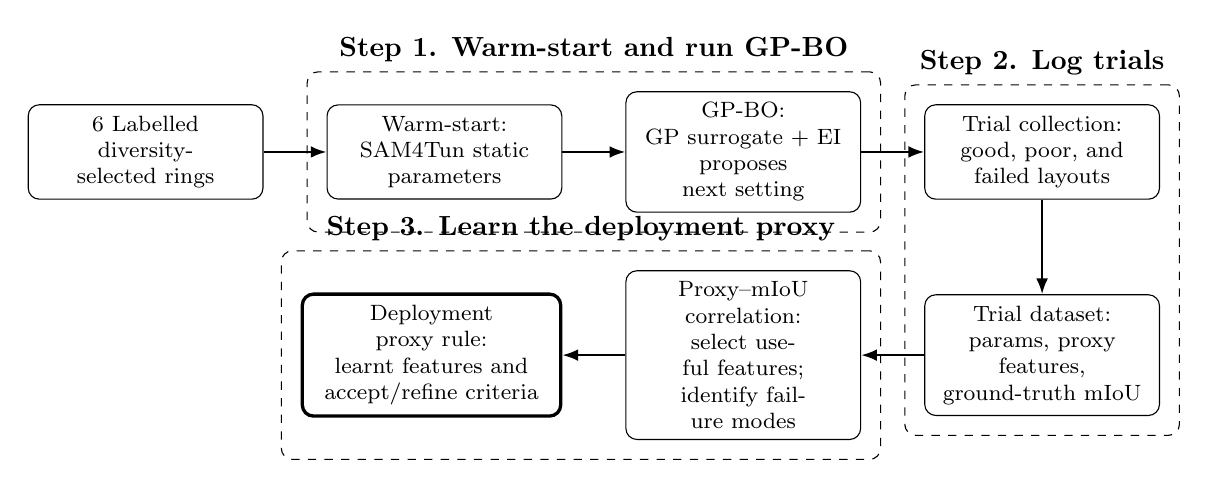
\begin{tikzpicture}[
    font=\footnotesize,
    box/.style={
        draw,
        rounded corners,
        align=center,
        minimum height=10mm,
        text width=27mm,
        inner sep=4pt
    },
    keybox/.style={
        draw,
        rounded corners,
        align=center,
        minimum height=10mm,
        text width=30mm,
        inner sep=4pt,
        very thick
    },
    stage/.style={
        draw,
        rounded corners,
        dashed,
        inner sep=7pt
    },
    arrow/.style={-{Latex[length=2mm]}, thick}
]

% Main flow nodes (wrapped into two stacks to fit page width)
% Top row
\node[box] (rings) at (0,0)
{6 Labelled\\diversity-selected rings};

\node[box, right=8mm of rings] (space)
{Warm-start:\\
{\footnotesize SAM4Tun static\\parameters}};

\node[box, right=8mm of space] (bo)
{GP-BO:\\
{\footnotesize GP surrogate + EI\\proposes next setting}};

\node[box, right=8mm of bo] (pool)
{Trial collection:\\
{\footnotesize good, poor, and\\failed layouts}};

% Bottom row (continues from pool, right-to-left)
\node[box, below=12mm of pool] (records)
{Trial dataset:\\
{\footnotesize params, proxy features,\\ground-truth mIoU}};

\node[box, left=8mm of records] (analysis)
{Proxy--mIoU\\correlation:\\
{\footnotesize select useful features;\\identify failure modes}};

\node[keybox, left=8mm of analysis] (proxy)
{Deployment\\proxy rule:\\
{\footnotesize learnt features and\\accept/refine criteria}};

% Arrows
\draw[arrow] (rings) -- (space);
\draw[arrow] (space) -- (bo);
\draw[arrow] (bo) -- (pool);
\draw[arrow] (pool) -- (records);
\draw[arrow] (records) -- (analysis);
\draw[arrow] (analysis) -- (proxy);

% Stage grouping boxes
\node[stage, fit=(space)(bo),
      label={[font=\bfseries]above:Step 1. Warm-start and run GP-BO}] (stage1) {};

\node[stage, fit=(pool)(records),
      label={[font=\bfseries]above:Step 2. Log trials}] (stage2) {};

\node[stage, fit=(analysis)(proxy),
      label={[font=\bfseries]above:Step 3. Learn the deployment proxy}] (stage3) {};

% Notes (removed for concision)

\end{tikzpicture}

\caption{
Design-time calibration of the deployment proxy. Six labelled diversity-selected rings are used to evaluate pipeline settings with Gaussian-process Bayesian optimisation (GP-BO): a Gaussian-process surrogate predicts the score (with uncertainty), and an Expected Improvement (EI) criterion proposes the next setting to test. Each trial saves a dataset comprising parameters, proxy features, and the ground-truth mIoU. These records are used to select effective proxy features and acceptance/refinement criteria, producing a learnt deployment proxy rule that operates without GT.
}
\label{fig:bo_proxy_calibration}
\end{figure*}
\FloatBarrier % keep Fig.~4 from floating past the equations/algorithm below
\clearpage % start the equations/algorithm at the top of a fresh left column (avoid an empty left column)


% Keep the two displayed equations together in the same column (no column break between them).
\par\noindent\begin{minipage}{\columnwidth}
\begin{equation}
\theta_{t+1}
= \arg\max_{\theta} \mathrm{EI}_t(\theta),
\qquad
\mathrm{EI}_t(\theta)
= \mathbb{E}\left[\max\left(s(\theta)-s_{\mathrm{best}},0\right)\right].
\label{eq:expected_improvement}
\end{equation}
where $\theta_0$ is the warm-start static setting, $s(\theta)$ is the calibration score for setting $\theta$, $\theta_{t+1}$ is the next setting chosen at BO iteration $t$, $\mathrm{EI}_t(\theta)$ is the Expected Improvement under the GP surrogate, and $s_{\mathrm{best}}$ is the best score observed so far. At iteration $t$, the GP surrogate models the score and uncertainty over candidates, and EI balances exploitation and exploration.

\begin{equation}
\rho_j
= \mathrm{Spearman}\!\left(
\{\phi_{i,j}\}_{i=1}^{N},
\{\mathrm{mIoU}^{GT}_{i}\}_{i=1}^{N}
\right),
\label{eq:proxy_miou_correlation}
\end{equation}
where $\rho_j$ is the Spearman rank correlation between proxy feature $\phi_j$ and ground-truth mIoU across the $N$ calibration trials (with $\phi_{i,j}$ and $\mathrm{mIoU}^{GT}_{i}$ from trial $i$). During calibration, $\phi_{i,j}$ is computed without labels, while $\mathrm{mIoU}^{GT}_{i}$ uses labels; only proxies with stable, interpretable correlation are kept for deployment.
\end{minipage}\par

% ─── Algorithm: Design-time calibration of the deployment proxy ───────────
\begin{algorithm}[t]
\caption{Design-time calibration of the deployment proxy}
\label{alg:design_time_proxy_calibration}
\begin{algorithmic}[1]
\Require Labelled diversity-selected rings, warm-start parameters $\theta_0$, tunable pipeline parameters, BO budget $T$
\Ensure Fixed deployment proxy rule
\State Initialise the trial set with the warm-start setting $\theta_0$
\For{$t=1,\ldots,T$}
    \State Run the ring-level pipeline with the current parameter setting
    \State Compute proxy features from the output layout without using labels
    \State Compute ground-truth mIoU for calibration only
    \State Update the Gaussian-process surrogate with the completed trial
    \State Select the next setting using Expected Improvement (Eq.~\ref{eq:expected_improvement})
\EndFor
\State Compute proxy--mIoU correlations for candidate proxy features (Eq.~\ref{eq:proxy_miou_correlation})
\State Select proxy features and accept/refine criteria
\State Freeze the selected features and criteria as the deployment proxy
\end{algorithmic}
\end{algorithm}

\FloatBarrier % ensure the equations+algorithm appear before Fig.~5

% ─── Figure (TikZ): Deployment-time refinement loop ───────────────────────
\begin{figure*}[t]
\centering
\resizebox{\textwidth}{!}{%
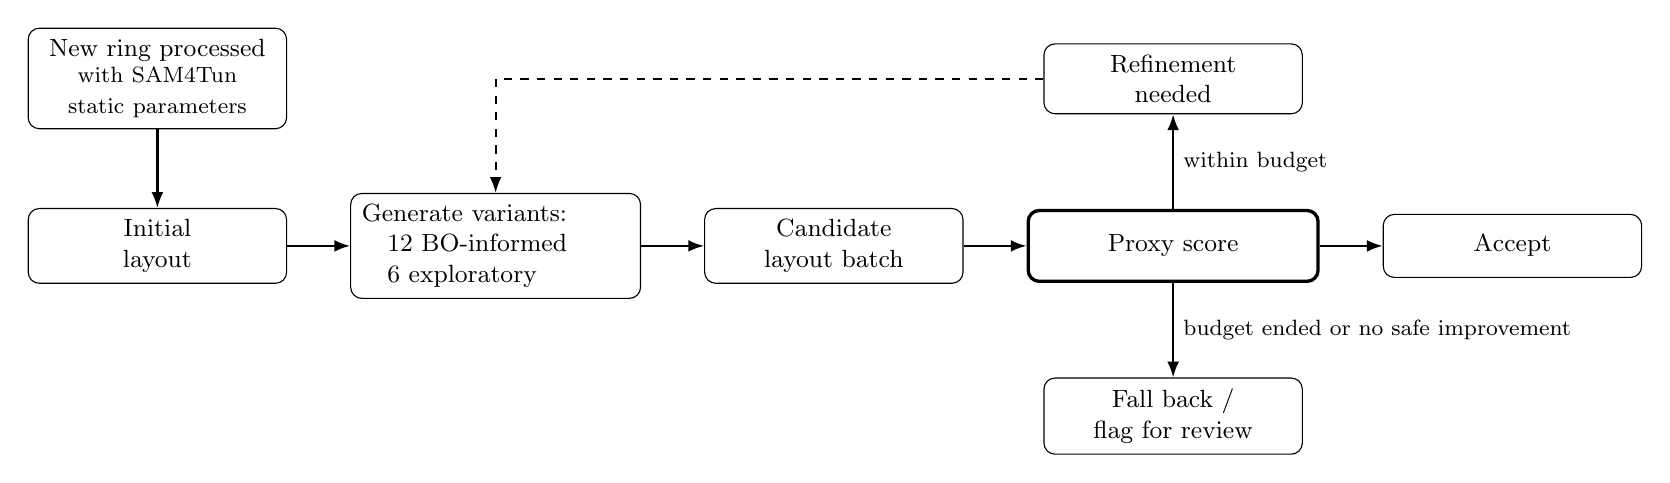
\begin{tikzpicture}[
    font=\small,
    box/.style={
        draw,
        rounded corners,
        align=center,
        minimum height=8mm,
        text width=30mm,
        inner sep=4pt
    },
    sbox/.style={
        draw,
        rounded corners,
        align=left,
        minimum height=8mm,
        text width=34mm,
        inner sep=4pt
    },
    gate/.style={
        draw,
        rounded corners,
        align=center,
        minimum height=9mm,
        text width=34mm,
        inner sep=4pt,
        very thick
    },
    arrow/.style={-{Latex[length=2mm]}, thick},
    looparrow/.style={-{Latex[length=2mm]}, thick, dashed}
]

% Horizontal deployment flow
\node[box] (initial) at (0,0)
{Initial\\layout};

% Move the "New ring" box above the main horizontal pipeline to free horizontal space.
\node[box, above=10mm of initial] (ring)
{New ring processed \\
{\footnotesize with SAM4Tun \\static parameters}};

\node[sbox, right=8mm of initial] (variants)
{Generate variants:\\
\quad 12 BO-informed\\
\quad 6 exploratory};

\node[box, right=8mm of variants] (batch)
{Candidate\\layout batch};

\node[gate, right=8mm of batch] (score)
{Proxy score};

\node[box, right=8mm of score] (selected)
{Accept};

\node[box, below=12mm of score] (fallback)
{Fall back /\\flag for review};

\node[box, above=12mm of score] (refine)
{Refinement\\needed};

\draw[arrow] (ring) -- (initial);
\draw[arrow] (initial) -- (variants);
\draw[arrow] (variants) -- (batch);
\draw[arrow] (batch) -- (score);
\draw[arrow] (score) -- (selected);
\draw[arrow] (score) -- node[right, font=\footnotesize]{budget ended or no safe improvement} (fallback);
\draw[arrow] (score) -- node[right, font=\footnotesize]{within budget} (refine);
\draw[looparrow] (refine.west) -- ++(-20mm,0) -| (variants.north);

\end{tikzpicture}
}
\caption{Deployment-time proxy-guided refinement and selection with a set candidate budget. Each new ring is first processed with the ring-level backbone initialised by the SAM4Tun static parameters. A variant generator produces 18 candidates: 12 BO-informed (concentrated near calibration-supported regions) and 6 exploratory (covering alternative possibilities). Each candidate is executed by the shared backbone to produce a layout, which is then evaluated by the learnt proxy score. The system accepts the best-scoring candidate, falls back to the initial layout and flags the ring when the budget ends or no improvement exists, or loops back to generate another batch when refinement is within budget.}
\label{fig:self_refinement}
\end{figure*}

\subsection{Datasets}\label{subsec:datasets}
\begin{table*}[t]
\caption{Composition of the BO calibration and evaluation panels. The BO panel contains six selected labelled rings used only at design time, while the evaluation panel contains 50 rings used for evaluation. Descriptors summarise point density, ring coverage, keystone span, and cyclic joint pattern diversity across the panels.}
\label{tab:dataset_panels}
\centering
\footnotesize
\begin{tabular}{lcc}
\toprule
Descriptor & BO calibration & evaluation \\
\midrule
Rings & 6 & 50 \\
Density (dense / medium / low) & 2 / 2 / 2 & 13 / 18 / 19 \\
Coverage (full / partial) & 5 / 1 & 48 / 2 \\
K-span (narrow / normal / wide) & 1 / 3 / 2 & 3 / 22 / 25 \\
Joint pattern (canonical / reversed canonical) & 3 / 3 & 26 / 24 \\
\bottomrule
\end{tabular}
\end{table*}

\subsection{Ablation design}\label{subsec:proxy_ablation_design}

\begin{figure*}[t]
\centering
\resizebox{\textwidth}{!}{%
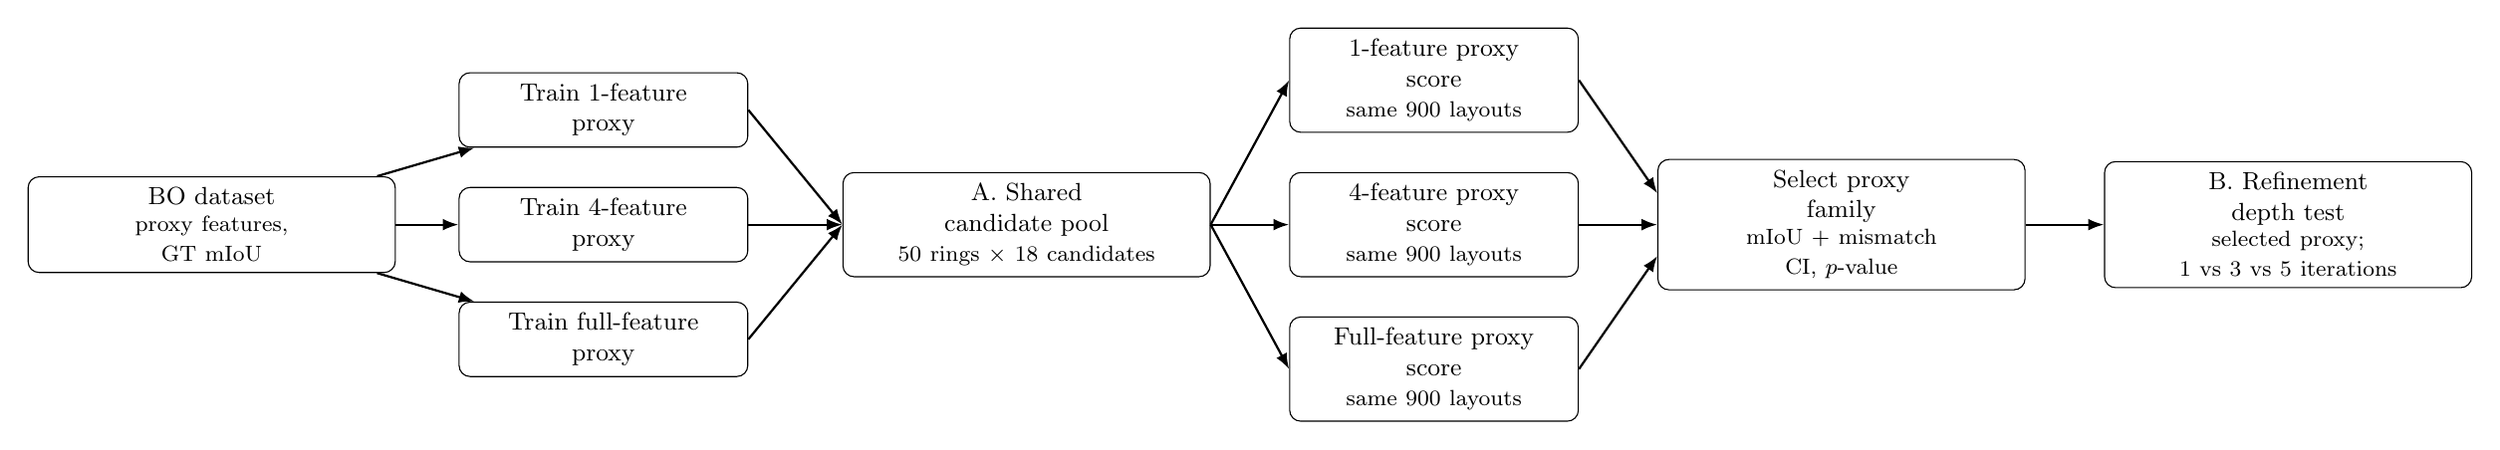
\begin{tikzpicture}[
    font=\small,
    box/.style={
        draw,
        rounded corners,
        align=center,
        minimum height=9mm,
        text width=34mm,
        inner sep=4pt
    },
    wide/.style={
        draw,
        rounded corners,
        align=center,
        minimum height=9mm,
        text width=44mm,
        inner sep=4pt
    },
    gate/.style={
        draw,
        rounded corners,
        align=center,
        minimum height=9mm,
        text width=38mm,
        inner sep=4pt,
        very thick
    },
    arrow/.style={-{Latex[length=2mm]}, thick}
]

\node[wide] (bo) at (0,0)
{BO dataset\\
{\footnotesize proxy features,\\GT mIoU}};

\node[box, right=8mm of bo] (p4)
{Train 4-feature\\proxy};
\node[box, above=5mm of p4] (p1)
{Train 1-feature\\proxy};
\node[box, below=5mm of p4] (pf)
{Train full-feature\\proxy};

\node[wide, right=12mm of p4] (pool)
{A. Shared\\candidate pool\\
{\footnotesize 50 rings $\times$ 18 candidates}};

% Score the same candidate pool with each proxy (split into three boxes)
\node[box, right=10mm of pool] (score4)
{4-feature proxy\\score\\
{\footnotesize same 900 layouts}};
\node[box, above=5mm of score4] (score1)
{1-feature proxy\\score\\
{\footnotesize same 900 layouts}};
\node[box, below=5mm of score4] (scoref)
{Full-feature proxy\\score\\
{\footnotesize same 900 layouts}};

\node[wide, right=10mm of score4] (select)
{Select proxy\\family\\
{\footnotesize mIoU + mismatch\\CI, $p$-value}};

\node[wide, right=10mm of select] (depth)
{B. Refinement\\depth test\\
{\footnotesize selected proxy;\\1 vs 3 vs 5 iterations}};

\draw[arrow] (bo) -- (p1);
\draw[arrow] (bo) -- (p4);
\draw[arrow] (bo) -- (pf);
\draw[arrow] (p1.east) -- (pool.west);
\draw[arrow] (p4.east) -- (pool.west);
\draw[arrow] (pf.east) -- (pool.west);
\draw[arrow] (pool.east) -- (score1.west);
\draw[arrow] (pool.east) -- (score4.west);
\draw[arrow] (pool.east) -- (scoref.west);

\draw[arrow] (score1.east) -- ([yshift=4mm]select.west);
\draw[arrow] (score4.east) -- (select.west);
\draw[arrow] (scoref.east) -- ([yshift=-4mm]select.west);
\draw[arrow] (select) -- (depth);

\end{tikzpicture}%
}
\caption{Two-stage ablation design. Stage A isolates proxy quality by training the three proxy families from the same six-ring BO archive and evaluating them on the same one-batch candidate layouts. Stage B fixes the proxy selected in Stage A and tests proxy-dependent self-refinement depth using 1, 3, and 5 refinement iterations.}
\label{fig:proxy_ablation_design}
\end{figure*}



\begin{table*}[t]
\caption{Ablation endpoints computed per evaluation ring before aggregation. The endpoints support three deployment interpretations: performance-dominant selection, safety-dominant selection, and opportunity-dominant selection.}
\label{tab:proxy_ablation_metrics}
\centering
\footnotesize
\begin{tabular}{p{0.22\textwidth}p{0.46\textwidth}p{0.22\textwidth}}
\toprule
Endpoint & Definition & Interpretation \\
\midrule
Selected mIoU & Ground-truth mIoU of the candidate selected by the proxy & Higher supports performance-dominant choice \\
Lift vs initial layout & Selected mIoU minus initial-layout mIoU & Higher paired lift supports performance-dominant choice \\
High-proxy / low-mIoU mismatch & Fraction of rings where the selected high-proxy candidate is below the initial-layout mIoU & Lower supports safety-dominant choice \\
Low-proxy / high-mIoU mismatch & Fraction of rings where the proxy falls back or selects no improvement while at least one candidate improves over the initial layout & Lower supports opportunity-dominant choice \\
\bottomrule
\end{tabular}
\end{table*}

\begin{table*}[t]
\caption{Decision rules used to interpret the proxy ablation. All comparisons are paired over evaluation rings and reported with 95\% confidence intervals and corrected paired $p$-values.}
\label{tab:proxy_ablation_interpretation}
\centering
\footnotesize
\begin{tabular}{p{0.24\textwidth}p{0.60\textwidth}}
\toprule
Deployment priority & Proxy selected by the ablation \\
\midrule
Maximum mIoU & \textbf{Choose proxy A.} Proxy with the highest selected mIoU or largest lift vs initial layout \\
Safety against bad selections & \textbf{Choose proxy B.} Proxy with the lowest high-proxy / low-mIoU mismatch, provided its lift is not statistically worse than the best-lift proxy \\
Capturing improvement opportunities & \textbf{Choose proxy C.} Proxy with the lowest low-proxy / high-mIoU mismatch, provided its high-proxy / low-mIoU mismatch is not higher \\
\bottomrule
\end{tabular}
\end{table*}

\begin{algorithm}[t]
\caption{Two-stage proxy and refinement-depth ablation}
\label{alg:proxy_ablation_shared_candidates}
\begin{algorithmic}[1]
\Require Six-ring BO archive, evaluation rings, proxy families in Table~\ref{tab:proxy_ablation_families}
\Ensure Selected proxy family and refinement-depth audit
\State For each proxy family, extract its feature columns from the BO archive
\State Impute missing feature values using the calibration-set median
\State Standardise features and fit Ridge regression ($\alpha=1.0$) to calibration mIoU
\Statex \textbf{Stage A: proxy-family ablation}
\For{each evaluation ring}
    \State Generate one shared 18-candidate batch: 12 BO-informed and 6 exploratory
    \State Execute the ring-level backbone once per candidate variant
    \For{each trained proxy}
        \State Score the same candidate layouts
        \State Select the best candidate by proxy score, or fall back to the initial layout
        \State Compute selected mIoU, lift, and the two proxy--mIoU mismatch rates
    \EndFor
\EndFor
\State Select the proxy family using the decision rules in Table~\ref{tab:proxy_ablation_interpretation}
\Statex \textbf{Stage B: refinement-depth ablation}
\For{each evaluation ring}
    \For{refinement budget in $\{1,3,5\}$}
        \State Run proxy-dependent refinement with the selected proxy and the given budget
        \State Compute selected mIoU, lift, and mismatch rates
    \EndFor
\EndFor
\State Compute paired ring-level differences for proxy families and refinement budgets
\State Estimate 95\% confidence intervals by bootstrap over rings
\State Compute paired $p$-values and apply multiplicity correction
\end{algorithmic}
\end{algorithm}

\FloatBarrier % keep Fig.~5 and ablation design artifacts from floating past the results section below
\clearpage
% ══════════════════════════════════════════════════════════════════════════
\section{Results}\label{sec:results}% ══════════════════════════════════════════════════════════════════════════
\subsection{Dataset and Candidate Pool}

\begin{table*}[t]
\caption{Evaluation panels and candidate records used by the visual results. The statistical unit for confidence intervals and paired tests is the ring. The Stage A artifacts reuse the available pilot candidate pool, while the final comparison uses the 50-ring heldout scoreboard.}
\label{tab:results_dataset_candidate_pool}
\centering
\footnotesize
\begin{tabular}{p{0.22\textwidth}p{0.22\textwidth}p{0.26\textwidth}p{0.22\textwidth}}
\toprule
Panel & Rings & Candidate records & Use \\
\midrule
Design-time BO archive & 6 labelled rings & offline calibration archive & proxy training and feature calibration \\
Stage A reused candidate pool & 16 calibration + 10 heldout rings & 150 candidate layouts & shared-candidate proxy-family ablation \\
Final heldout panel & 50 rings & one selected output per ring plus oracle/reference columns & final method comparison \\
\bottomrule
\end{tabular}

\end{table*}

\begin{table*}[t]
\caption{Artifact provenance for the visual-only Results section. ``Reused'' denotes a prior run output read directly from disk, ``derived'' denotes a chart or table computed from a prior CSV, and ``pending'' denotes a planned visual slot for which no completed run output was found.}
\label{tab:results_artifact_provenance}
\centering
\scriptsize
\begin{tabular}{p{0.23\textwidth}p{0.38\textwidth}p{0.12\textwidth}p{0.18\textwidth}}
\toprule
Result artifact & Source CSV & Status & Manuscript slot \\
\midrule
Candidate mIoU distribution & \texttt{logs/v6\_proxy\_ablation\_study\_v1/candidate\_pool.csv} & reused & Fig.~\ref{fig:candidate_miou_distribution} \\
Stage A proxy lift & \texttt{logs/v6\_proxy\_ablation\_study\_v1/proxy\_ablation\_results\_by\_ring.csv} & reused & Fig.~\ref{fig:stage_a_proxy_lift} \\
Stage A mismatch & \texttt{logs/v6\_proxy\_ablation\_study\_v1/proxy\_ablation\_results\_by\_ring.csv} & derived & Fig.~\ref{fig:stage_a_proxy_mismatch} \\
Stage A pairwise tests & \texttt{logs/v6\_proxy\_ablation\_study\_v1/proxy\_pairwise\_tests.csv} & reused & Table~\ref{tab:stage_a_pairwise_tests} \\
Stage B 1/3/5 depth & \texttt{not found in prior outputs} & pending & Figs.~\ref{fig:stage_b_refinement_depth}--\ref{fig:stage_b_mismatch_depth} \\
Final 50-ring comparison & \texttt{logs/v7\_diverse\_calibration\_restart/imported\_v5\_prior/selected\_scoreboard\_50rings.csv} & reused & Fig.~\ref{fig:final_selected_vs_initial} \\
\bottomrule
\end{tabular}

\end{table*}

\begin{figure*}[t]
\centering
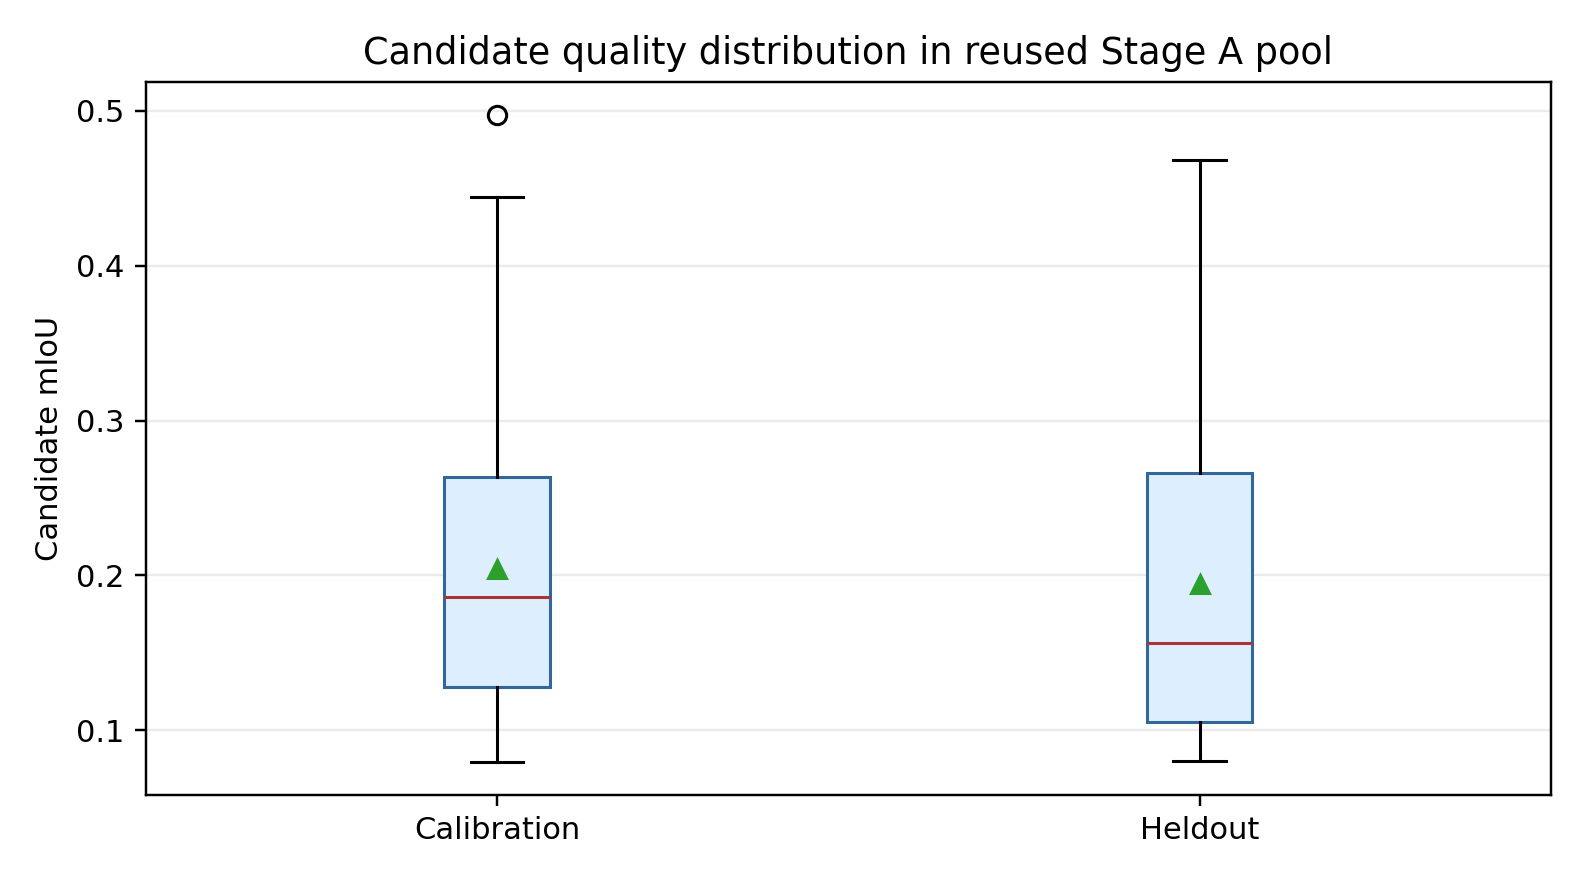
\includegraphics[width=0.72\textwidth]{figures/results_candidate_miou_distribution.png}
\caption{Candidate mIoU distribution in the reused Stage A candidate pool. Boxes summarise candidate layouts by split; the available artifact contains 16 calibration rings and 10 heldout rings, with 150 candidate layouts in total.}
\label{fig:candidate_miou_distribution}
\end{figure*}

\subsection{Stage A: Proxy-Family Ablation}

\begin{table*}[t]
\caption{Proxy families compared in Stage A. Each proxy is trained as a median-imputed, standardised Ridge regression on calibration mIoU. The full-feature family is the predefined proxy-feature library recorded for every candidate layout; BO calibration is used to fit the proxy weights, not to define this feature list from evaluation results.}
\label{tab:proxy_ablation_families}
\centering
\footnotesize
\begin{tabular}{p{0.20\textwidth}p{0.18\textwidth}p{0.52\textwidth}}
\toprule
Proxy family & Scope & Proxy features \\
\midrule
Single-feature & one feature
& \texttt{balance\_norm} \\
\addlinespace
Compact descriptor & four features
& \texttt{anchor\_frac}, \texttt{low\_parity}, \texttt{regular\_k\_prior\_low\_frac}, \texttt{regular\_k\_prior\_high\_frac} \\
\addlinespace
Full proxy-feature library & all recorded features
& \texttt{struct\_missing\_ids\_before\_n}, \texttt{depth\_row\_nonempty\_ratio\_audit}, \texttt{geom\_boundary\_gap\_cv}, \texttt{present\_ratio}, \texttt{entropy}, \texttt{cv}, \texttt{max\_share}, \texttt{balance\_norm}, \texttt{anchor\_frac}, \texttt{low\_parity}, \texttt{regular\_k\_prior\_low\_frac}, \texttt{regular\_k\_prior\_high\_frac}, \texttt{rotation\_shift\_num} \\
\bottomrule
\end{tabular}
\end{table*}

\begin{figure*}[t]
\centering
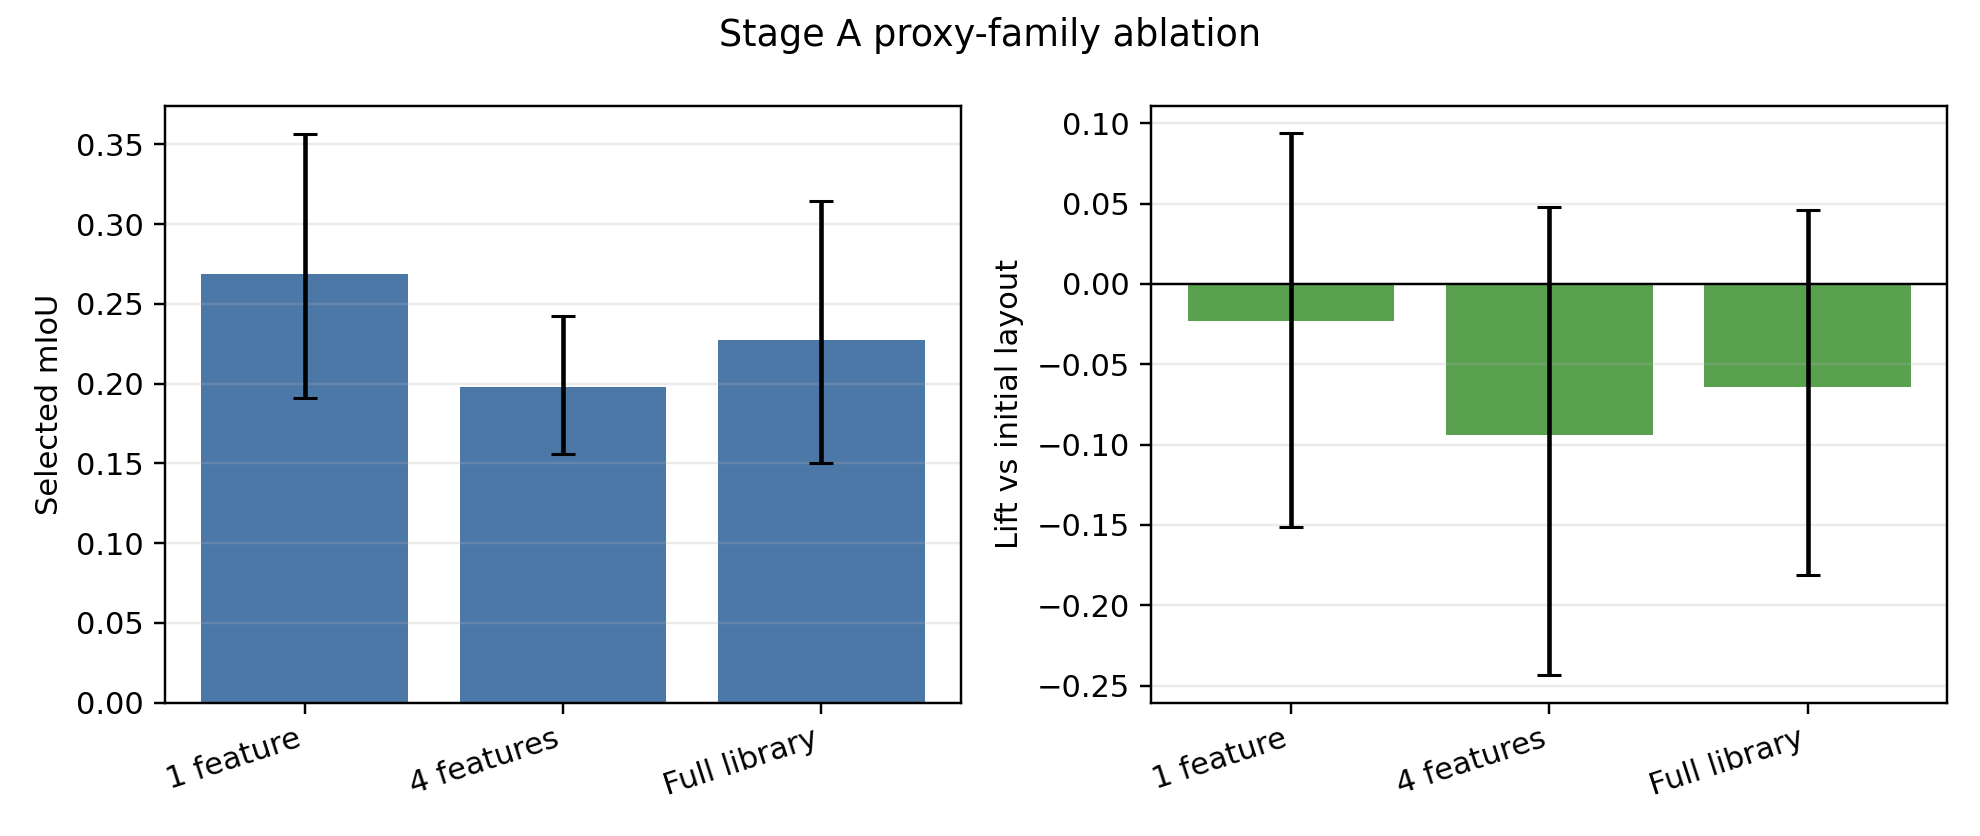
\includegraphics[width=0.88\textwidth]{figures/stage_a_proxy_lift.png}
\caption{Stage A proxy-family ablation on the available 10-ring heldout artifact. Bars show mean selected mIoU and lift relative to the initial layout; error bars are 95\% bootstrap confidence intervals over rings.}
\label{fig:stage_a_proxy_lift}
\end{figure*}

\begin{figure*}[t]
\centering
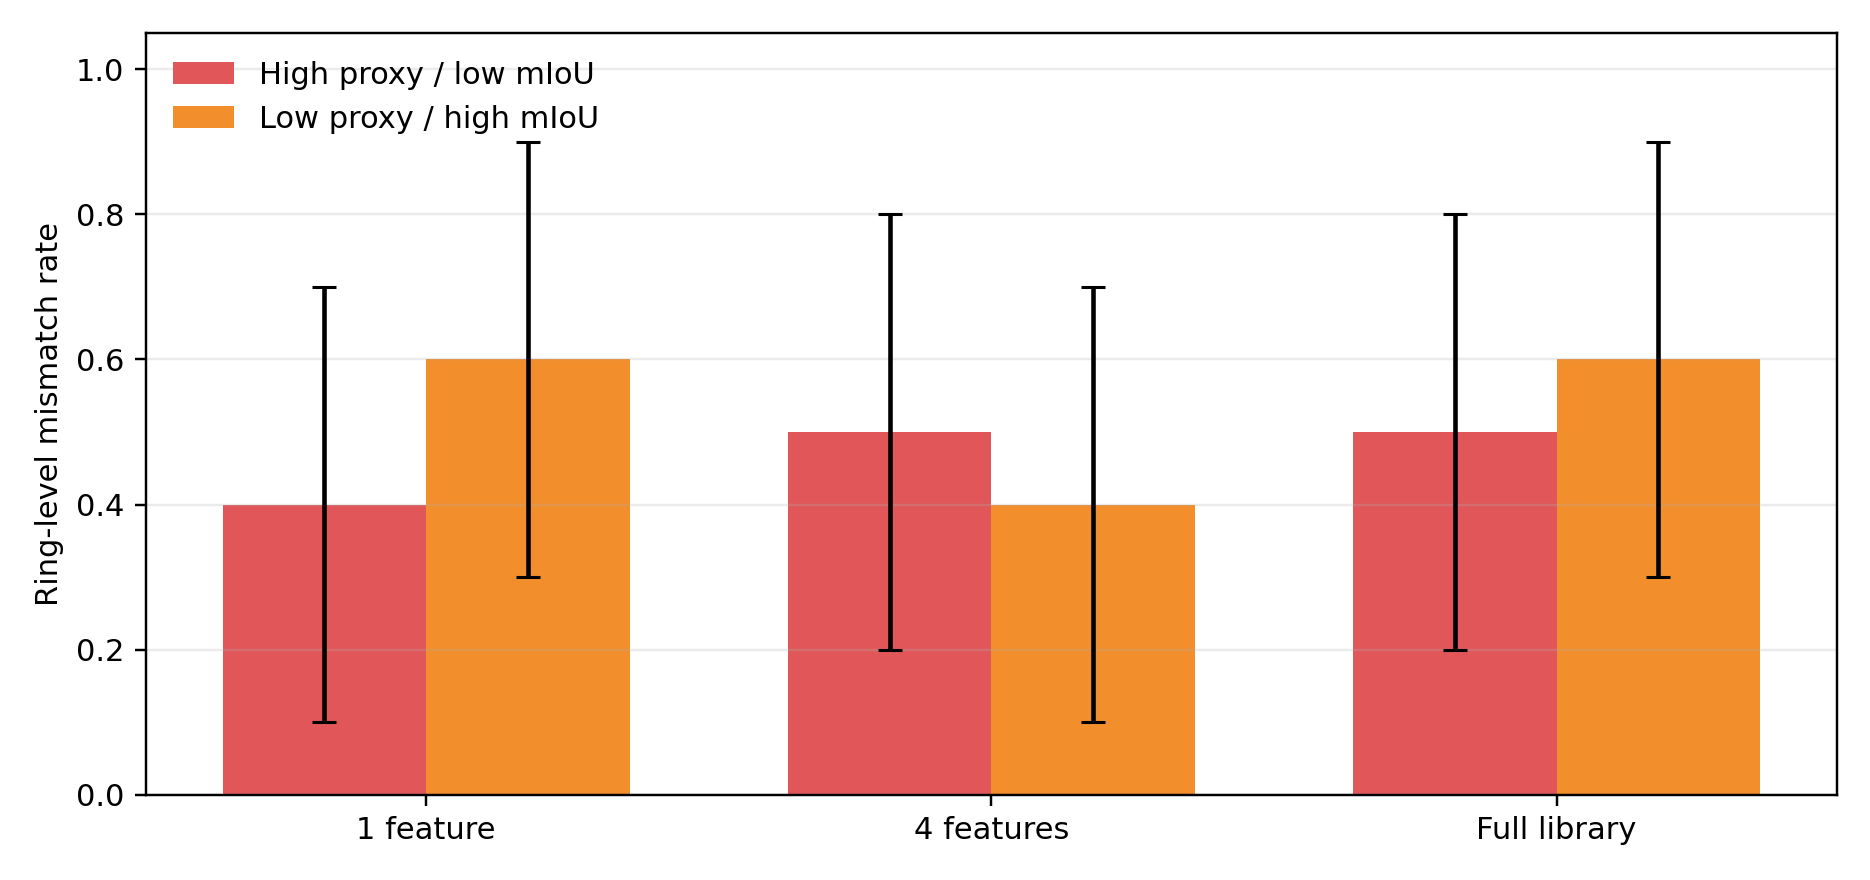
\includegraphics[width=0.82\textwidth]{figures/stage_a_proxy_mismatch.png}
\caption{Proxy--mIoU mismatch rates for the same Stage A heldout rings as Fig.~\ref{fig:stage_a_proxy_lift}. High-proxy/low-mIoU denotes a proxy-selected candidate below the initial layout; low-proxy/high-mIoU denotes a ring where the oracle candidate improves over the initial layout but is not selected by the proxy. Error bars are 95\% bootstrap confidence intervals over rings.}
\label{fig:stage_a_proxy_mismatch}
\end{figure*}

\begin{table*}[t]
\caption{Stage A numerical summary for the three target proxy families. Metrics are averaged over the available heldout rings; mismatch definitions match Fig.~\ref{fig:stage_a_proxy_mismatch}.}
\label{tab:stage_a_summary_metrics}
\centering
\footnotesize
\begin{tabular}{p{0.22\textwidth}cccc}
\toprule
Proxy family & Selected mIoU & Lift & High/low mismatch & Low/high mismatch \\
\midrule
1 feature & 0.269 & -0.023 & 40.0\% & 60.0\% \\
4 features & 0.198 & -0.094 & 50.0\% & 40.0\% \\
Full library & 0.228 & -0.064 & 50.0\% & 60.0\% \\
\bottomrule
\end{tabular}

\end{table*}

\begin{table*}[t]
\caption{Paired Stage A comparisons among the initial layout and the three proxy families. Mean differences are computed ring-wise on selected mIoU; $p$-values use paired permutation tests and Holm correction across the reported comparisons.}
\label{tab:stage_a_pairwise_tests}
\centering
\footnotesize
\begin{tabular}{p{0.43\textwidth}ccc}
\toprule
Comparison & Mean difference & $p$ & Holm $p$ \\
\midrule
Initial vs 1 feature & 0.023 & 0.734 & 1.000 \\
Initial vs Full library & 0.064 & 0.331 & 1.000 \\
Initial vs 4 features & 0.094 & 0.268 & 1.000 \\
1 feature vs Full library & 0.041 & 0.028 & 1.000 \\
1 feature vs 4 features & 0.071 & 0.246 & 1.000 \\
Full library vs 4 features & 0.030 & 0.610 & 1.000 \\
\bottomrule
\end{tabular}

\end{table*}

\subsection{Stage B: Refinement-Depth Ablation}

\begin{figure*}[t]
\centering
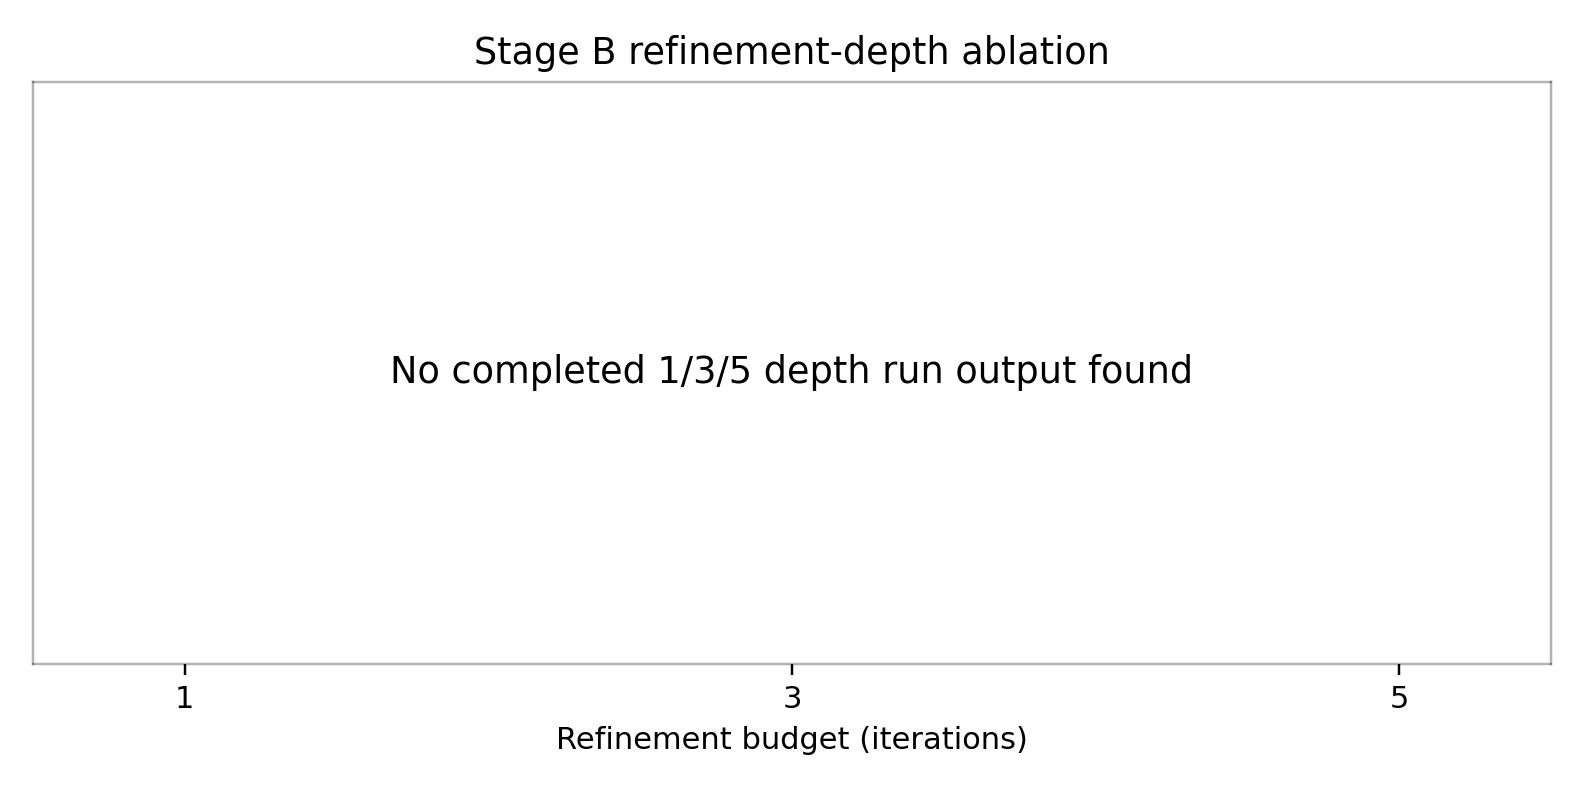
\includegraphics[width=0.70\textwidth]{figures/stage_b_refinement_depth.png}
\caption{Planned Stage B selected-mIoU chart for refinement budgets of 1, 3, and 5 iterations. The visual slot is included to preserve the Results layout; no completed 1/3/5 refinement-depth run output was found among the reusable artifacts, so no mean, confidence interval, or paired test is reported here.}
\label{fig:stage_b_refinement_depth}
\end{figure*}

\begin{figure*}[t]
\centering
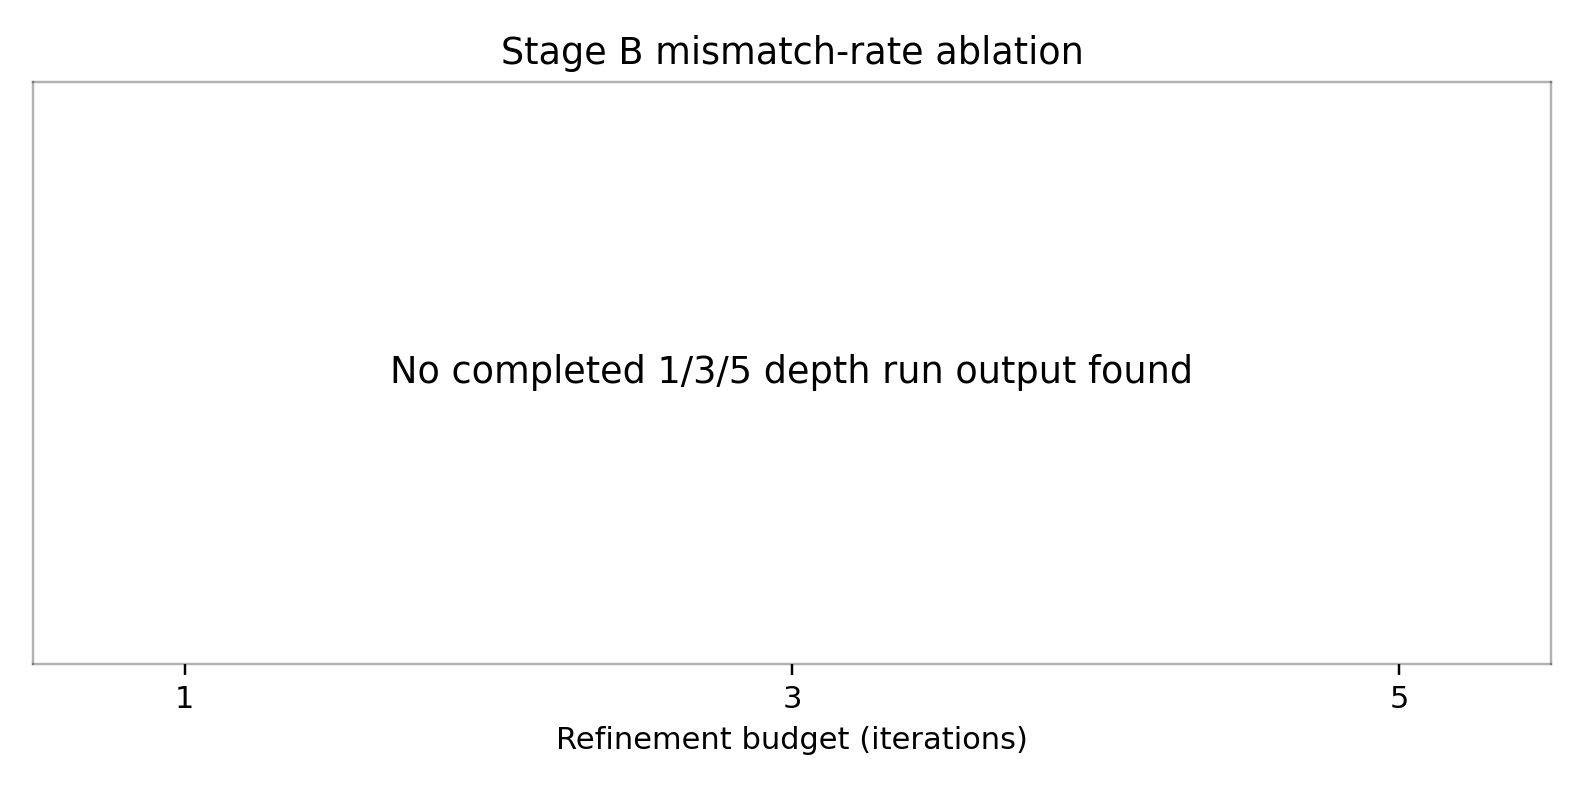
\includegraphics[width=0.70\textwidth]{figures/stage_b_mismatch_depth.png}
\caption{Planned Stage B mismatch-rate chart for refinement budgets of 1, 3, and 5 iterations. The statistical unit remains the ring, but the required depth-ablation CSV is not available in the prior outputs.}
\label{fig:stage_b_mismatch_depth}
\end{figure*}

\begin{table*}[t]
\caption{Planned paired comparisons for Stage B. The comparisons are defined before running the depth study; cells remain blank until the 1-, 3-, and 5-iteration outputs are produced on the same ring panel.}
\label{tab:stage_b_pairwise_tests}
\centering
\footnotesize
\begin{tabular}{p{0.30\textwidth}ccc}
\toprule
Budget comparison & Mean difference & $p$ & Holm $p$ \\
\midrule
1 vs 3 iterations & -- & -- & -- \\
3 vs 5 iterations & -- & -- & -- \\
1 vs 5 iterations & -- & -- & -- \\
\bottomrule
\end{tabular}

\end{table*}

\subsection{Proxy Conflict Diagnostics}

\begin{table*}[t]
\caption{Representative Stage A proxy--mIoU conflict examples. Selected, initial, and oracle columns report ground-truth mIoU for diagnosis only; the proxy itself does not use these labels at deployment.}
\label{tab:proxy_conflict_examples}
\centering
\scriptsize
\begin{tabular}{p{0.14\textwidth}p{0.12\textwidth}p{0.21\textwidth}p{0.15\textwidth}ccc}
\toprule
Ring & Proxy & Mismatch type & Selected candidate & Selected & Initial & Oracle \\
\midrule
1-5/r270 & 1 feature & High proxy / low mIoU & c02 & 0.140 & 0.535 & 0.216 \\
5-7/r317 & 1 feature & Low proxy / high mIoU & c04 & 0.088 & 0.425 & 0.287 \\
1-5/r270 & 4 features & High proxy / low mIoU & c01 & 0.112 & 0.535 & 0.216 \\
3-1-3/r86 & 4 features & Low proxy / high mIoU & c01 & 0.103 & 0.463 & 0.469 \\
1-5/r270 & Full library & High proxy / low mIoU & c02 & 0.140 & 0.535 & 0.216 \\
5-7/r317 & Full library & Low proxy / high mIoU & c02 & 0.086 & 0.425 & 0.287 \\
\bottomrule
\end{tabular}

\end{table*}

\subsection{Final Method Choice}

\begin{table*}[t]
\caption{Proxy choice implied by the Stage A visual diagnostics under different deployment priorities. The table separates performance, safety, and opportunity criteria so that the selected proxy can be justified by the deployment objective rather than by mean mIoU alone.}
\label{tab:proxy_decision_summary}
\centering
\footnotesize
\begin{tabular}{p{0.30\textwidth}p{0.20\textwidth}p{0.40\textwidth}}
\toprule
Deployment priority & Proxy choice & Decision rule \\
\midrule
Maximum mIoU & 1 feature & highest mean selected mIoU in Stage A \\
Safety against bad selections & 1 feature & lowest high-proxy/low-mIoU mismatch rate \\
Capturing improvement opportunities & 4 features & lowest low-proxy/high-mIoU mismatch rate \\
Balanced default & 1 feature & best selected mIoU among the three target families \\
\bottomrule
\end{tabular}

\end{table*}

\begin{figure*}[t]
\centering
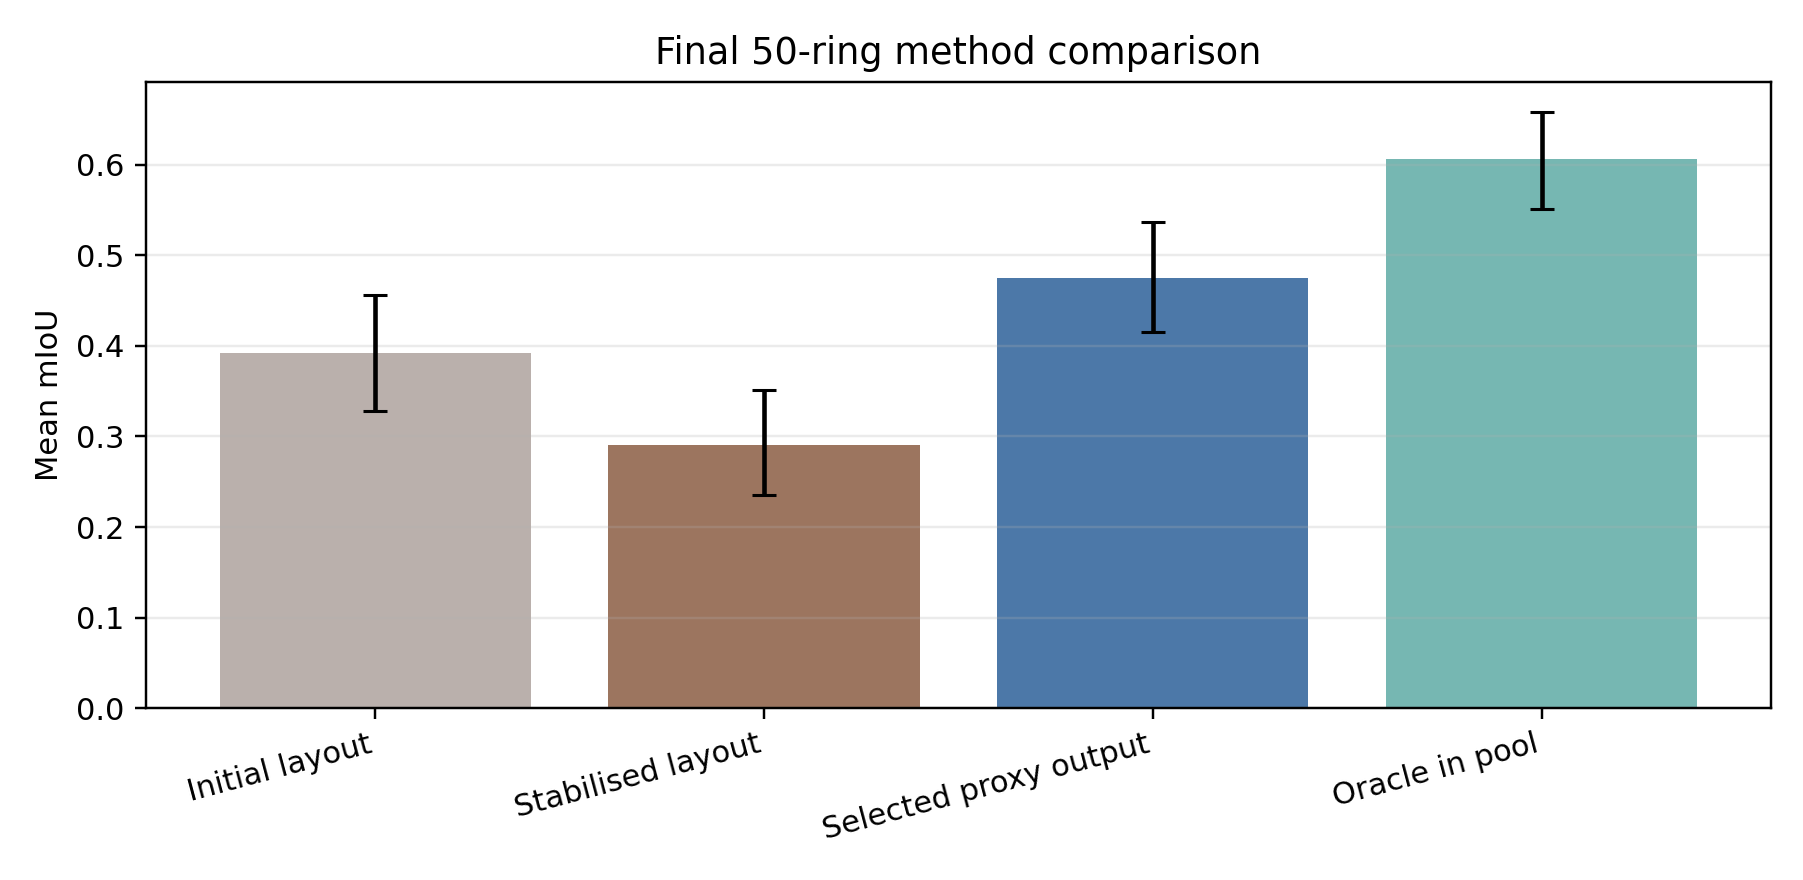
\includegraphics[width=0.78\textwidth]{figures/final_selected_vs_initial.png}
\caption{Final 50-ring method comparison from the reused heldout scoreboard. Bars show mean mIoU for the initial layout, stabilised layout, selected proxy output, and oracle candidate in the available pool; error bars are 95\% bootstrap confidence intervals over rings.}
\label{fig:final_selected_vs_initial}
\end{figure*}

\begin{table*}[t]
\caption{
Candidate-variant parameters scored by the deployment proxy.
Each group controls one mechanism used to generate alternative ring-level layouts from the same input ring.
}
\label{tab:workflow_critical_parameters}
\centering
\footnotesize
\begin{tabular}{p{0.20\textwidth}p{0.36\textwidth}p{0.36\textwidth}}
\toprule
Stage & Parameters & Definition / effect on the pipeline \\
\midrule
Ring extraction / cylindrical reference
& \texttt{tunnel\_diameter}
& Sets the cylindrical scale used when unfolding the ring and generating candidate variants. \\
\addlinespace
Bottom-aligned unfolding
& --
& Preset bottom alignment is applied before candidate generation; no unfolding parameter is varied in the candidate set. \\
\addlinespace
Radial point filtering
& \texttt{radius\_min}, \texttt{outlier\_neighbors}
& Adjust the lower radial acceptance limit and local-neighbour support used in filtering/cleanup variants. \\
\addlinespace
Curvature-guided upsampling
& \texttt{interpolation\_window}
& Adjusts the local interpolation window used when densifying sparse or missing lining support. \\
\addlinespace
Boundary and layout detection
& \texttt{anchor\_frac}, \texttt{half\_window}, \texttt{low\_parity}, \texttt{regular\_k\_prior\_low\_frac}, \texttt{regular\_k\_prior\_high\_frac}, \texttt{rotation\_shift}
& Adjust K-anchor location, branch/order hypothesis, K-prior interval, and rotation alternative used to produce candidate layouts. \\
\bottomrule
\end{tabular}
\end{table*}
% ══════════════════════════════════════════════════════════════════════════
\section{Discussion}\label{sec:discussion}
% ══════════════════════════════════════════════════════════════════════════

% ══════════════════════════════════════════════════════════════════════════
\section{Conclusions}\label{sec:conclusions}
% ══════════════════════════════════════════════════════════════════════════

% ══════════════════════════════════════════════════════════════════════════
% Data availability, declarations, etc.
% ══════════════════════════════════════════════════════════════════════════

\section*{Data availability}

The source code, adapted parameters, and evaluation scripts are available at \url{https://github.com/Tao-Robominds/R4Tun}. The Seg2Tunnel dataset is publicly available.

\section*{Declaration of competing interest}

The authors declare that they have no known competing financial interests or personal relationships that could have appeared to influence the work reported in this paper.

%\printcredits  % Uncomment if cas-dc supports it in your version

% ══════════════════════════════════════════════════════════════════════════
% Appendices
% ══════════════════════════════════════════════════════════════════════════

% \clearpage
\section*{Appendices}

% \input{appendices}


% ══════════════════════════════════════════════════════════════════════════
% Bibliography
% ══════════════════════════════════════════════════════════════════════════

% \clearpage % start Biography on a new page
% \section*{Biography}

\end{document}
